\chapter{Software Stack in HPC}
L'utilizzo di un cluster HPC differisce radicalmente da quello di un normale PC o di un server tradizionale.
La necessità di introdurre uno stack software specifico nasce da tre fattori chiave:
\begin{itemize}
    \item \textbf{La natura delle risorse: } I sistemi HPC mettono a disposizione risorse (CPU, memoria, rete e storage) che sono per definizione condivise, estremamente costose e spesso destinate a task critici.
    \item \textbf{La competizione:} A differenza di un PC personale, in un cluster ci sono costantemente molti utenti che competono per utilizzare queste stesse risorse nello stesso momento.
    \item \textbf{Il rischio del caos:} Senza un livello software in grado di orchestrare tutto questo, i risultati sarebbero disastrosi, portando a:
        \begin{itemize}
            \item Spreco di risorse (es. nodi lasciati inattivi o sovraccaricati).
            \item Conflitti tra utenti (programmi che si "rubano" memoria a vicenda o si bloccano).
            \item Impossibilità di garantire le prestazioni previste e l'equità (fairness) nell'accesso al sistema da parte di tutti.
        \end{itemize}
\end{itemize}

 
La regola d'oro è che \textbf{ogni livello interagisce con quelli adiacenti e influenza il comportamento prestazionale dell'intero sistema}.

\begin{figure}[H]
    \centering
    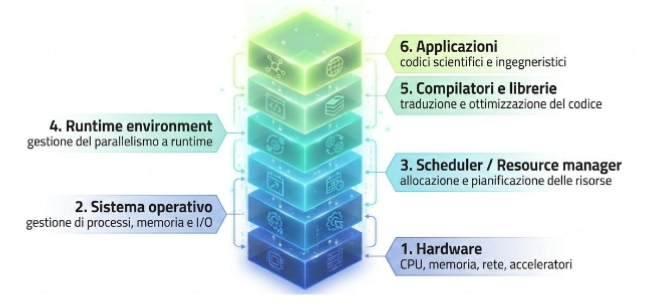
\includegraphics[width=0.85\linewidth]{Images/cap_1/stack_HPC.png}
\end{figure}

Partendo dalle fondamenta fisiche e salendo fino all'utente, troviamo 6 livelli:
\begin{itemize}
    \item \textbf{1. Hardware}: costituisce la base fisica (CPU, memoria, rete, acceleratori).
    \item \textbf{2. Sistema operativo}: si occupa della gestione di base dei processi, della memoria e dell'I/O.
    \item \textbf{3. Scheduler / Resource manager}: è il livello responsabile dell'allocazione e lo \textbf{scheduling} delle risorse del cluster.
    \item \textbf{4. Runtime environment}: gestisce il parallelismo a runtime durante l'esecuzione vera e propria.
    \item \textbf{5. Compilatori e librerie}: sono fondamentali per la traduzione e, soprattutto, l'ottimizzazione del codice affinché sfrutti l'hardware.
    \item \textbf{6. Applicazioni}: rappresentano i programmi finali, come i codici scientifici e ingegneristici degli utenti.
\end{itemize}

Dal punto di vista dell'utente, un sistema HPC non deve essere visto come una singola macchina, bensì come un vero e proprio \textbf{ambiente di calcolo controllato}.

Esso rappresenta, infatti, l'integrazione strutturata di hardware, software e specifiche \textbf{policy di utilizzo}. L'intera infrastruttura è stata pensata e progettata con il duplice scopo di eseguire \textbf{job di lunga durata} e di \textbf{massimizzare l'utilizzo complessivo} delle risorse a disposizione. 
Trattandosi di un sistema intrinsecamente \textbf{condiviso}, è importante tenere a mente che le risorse hardware non sono sempre immediatamente disponibili. Di conseguenza, l'accesso alla potenza di calcolo non avviene in modo diretto, ma è sempre \textbf{mediato}: l'utente interagisce inizialmente solo con un nodo di accesso detto \textbf{nodo di Login} che si occuperà di gestire le richieste al cluster di calcolo vero e proprio.

Il \textbf{Login Node} funge da punto di accesso interattivo per gli utenti le attività consentite su questa macchina si limitano alla preparazione del lavoro, come l'editing del codice, la sua eventuale compilazione e l'impostazione dei job. È fondamentale ricordare che questo nodo \textbf{non è destinato all'esecuzione di calcoli}. Al contrario, i \textbf{Compute Node} sono le vere e proprie risorse dedicate al calcolo puro. L'accesso a questi nodi non è mai diretto, ma avviene sempre in modo mediato: essi si occupano dell'esecuzione dei job batch e sono utilizzabili esclusivamente in seguito all'assegnazione di un job da parte dello \textbf{scheduler}. 

\begin{figure}[H]
    \centering
    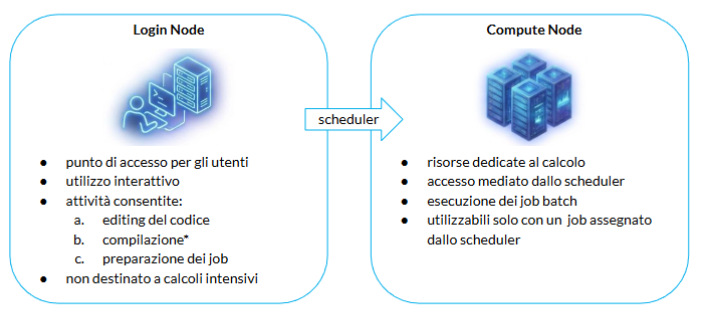
\includegraphics[width=0.85\linewidth]{Images/cap_1/login_vs_compute.png}
\end{figure}

Questa rigida separazione non è casuale, ma rappresenta una scelta architetturale obbligata per gestire e proteggere un hardware estremamente costoso. Nello specifico, isolare le attività di preparazione (spesso interattive e imprevedibili) da quelle di calcolo serve a garantire la \textbf{stabilità} dell'intero sistema e a proteggere le risorse computazionali. 
Inoltre, questa barriera impedisce che le operazioni o gli errori di un singolo utente possano causare interferenze con i lavori in esecuzione degli altri, assicurando un utilizzo \textbf{equo ed efficiente} delle macchine e permettendo allo scheduler di effettuare una pianificazione controllata e ottimale dei job.

\section{Filesystem nei sistemi HPC}

La gestione dei dati all'interno dei sistemi HPC è affidata a un \textbf{filesystem condiviso} tra i login node e i compute node, garantendo così che i dati siano accessibili contemporaneamente da molti nodi.  Questa infrastruttura è appositamente progettata per offrire un \textbf{elevato throughput} e per supportare \textbf{accessi paralleli}, motivo per cui viene spesso implementata come un vero e proprio \textbf{filesystem parallelo}. A livello pratico, gli utenti interagiscono principalmente con due directory tipiche: la \texttt{\$HOME}, dedicata alla conservazione dei dati personali e dei file di configurazione, e la \texttt{\$SCRATCH}, pensata appositamente per ospitare i dati temporanei e per memorizzare l'output generato dai job in esecuzione.

Le modalità con cui le applicazioni effettuano le operazioni di Input/Output (I/O) hanno un impatto diretto e profondo sulle prestazioni e sulla scalabilità dell'intero sistema. Ad esempio, l'elaborazione di \textbf{molti file di piccole dimensioni} comporta un elevato overhead, il quale si traduce in una forte degradazione delle prestazioni globali. Analogamente, gli \textbf{accessi casuali} in memoria penalizzano sia il throughput che la latenza, non riuscendo a sfruttare l'ottimizzazione offerta dalla struttura del filesystem parallelo. 
er poter gestire grandi volumi di dati in maniera efficiente, è strettamente necessario ricorrere all'\textbf{I/O parallelo}, che garantisce un accesso coordinato ai file da parte di molteplici processi contemporaneamente. In conclusione, la gestione dell'I/O rappresenta molto spesso il \textbf{vero limite alla scalabilità} di un programma, persino in quegli scenari in cui la componente di puro calcolo riesce a scalare in modo perfettamente corretto.

\section{Compilatori in ambienti HPC}
In un ambiente HPC sono tipicamente messi a disposizione degli utenti molteplici \textbf{compilatori}, tra cui troviamo le opzioni più note come GCC o Clang/LLVM, affiancate spesso da compilatori \textbf{vendor-specific} (come quelli forniti da Intel, AOCC o NVIDIA HPC). Il ruolo del compilatore va ben oltre la semplice traduzione del codice sorgente poiché si occupa di applicare \textbf{ottimizzazioni automatiche} e di generare un codice che sia specificamente ottimizzato per l'architettura su cui andrà in esecuzione. Per questo motivo, il compilatore non è un semplice strumento di traduzione, ma deve essere considerato a tutti gli effetti come \textbf{parte integrante delle prestazioni} finali di un'applicazione.

La ragione per cui all'interno di questi sistemi coesistono più compilatori è dovuta in primis alla grande diversità delle \textbf{architetture hardware} sottostanti. Ogni compilatore implementa, infatti, differenti \textbf{strategie di ottimizzazione} e gestisce in modo diverso i modelli di vettorizzazione e di parallelismo. Inoltre, è frequente che determinate librerie risultino maggiormente ottimizzate solo se trattate con compilatori specifici. 
Nella pratica, chi sviluppa si trova spesso a dover gestire una naturale \textbf{tensione} tra la massima portabilità del codice e la ricerca delle massime prestazioni. Proprio per questo motivo, è fondamentale ricordare che \textbf{non esiste un compilatore "migliore" in assoluto}, ma bisogna saper scegliere quello più adatto al proprio caso d'uso e al proprio hardware.

È bene segnalare che si potrebbe provare a compilare il codice con più compilatori per vedere quale ci ritorna delle prestazioni migliori.
\section{Librerie}
Nei sistemi HPC, le \textbf{librerie} rappresentano dei componenti centrali dell'intero stack software, in quanto forniscono implementazioni già ampiamente ottimizzate per le operazioni fondamentali. Il loro grande vantaggio è quello di incapsulare al loro interno sia una profonda conoscenza dell'architettura hardware sia le ottimizzazioni più avanzate, tanto che spesso determinano le prestazioni finali molto più di quanto non faccia il codice applicativo stesso. Tra gli esempi più importanti a disposizione degli sviluppatori troviamo:
\begin{itemize}
    \item \textbf{MPI}: fondamentale per gestire la comunicazione tra processi in sistemi a memoria distribuita.
    \item \textbf{OpenMP}: standard di fatto per gestire il parallelismo in architetture a memoria condivisa.
    \item \textbf{BLAS / LAPACK}: librerie di base, essenziali per le operazioni di algebra lineare.
\end{itemize}

Questa enorme ricchezza di strumenti, tuttavia, genera il cosiddetto \textbf{problema dell'ambiente software}. Rispetto a un computer classico, l'ambiente di un cluster HPC è intrinsecamente molto più complesso. Su queste macchine devono \textbf{necessariamente coesistere molteplici versioni di compilatori e innumerevoli versioni delle stesse librerie}, poiché le varie applicazioni degli utenti presentano dipendenze specifiche e requisiti spesso incompatibili tra loro. Un concetto fondamentale da tenere a mente è che il compilatore altera il risultato finale ad esempio una libreria MPI compilata con GCC è incompatibile e profondamente diversa da una compilata con strumenti Intel. Diventa quindi imperativo che l'ambiente sia sempre controllato, riproducibile e configurabile dinamicamente per ogni singolo utente e per ogni specifico job.

La soluzione standard adottata universalmente nei sistemi HPC per domare questa complessità prende il nome di \textbf{Environment Modules}. Si tratta di un meccanismo che permette di "caricare" dinamicamente solo le versioni specifiche del software necessario per il proprio lavoro, configurando l'ambiente su misura. All'atto pratico, i moduli agiscono andando a modificare in modo sicuro le variabili d'ambiente del sistema operativo (come ad esempio i percorsi \texttt{PATH} o \texttt{LD\_LIBRARY\_PATH}). Questo approccio elegante garantisce la coesistenza pacifica di più compilatori e versioni dello stesso software, favorendo al contempo un elevato grado di controllo, grande flessibilità e, soprattutto, la totale riproducibilità degli esperimenti 

\section{Scheduler}
Il \textbf{runtime environment} rappresenta il livello software responsabile della gestione e dell'esecuzione di un programma parallelo a tempo di run-time. Pur non facendo parte del kernel del sistema operativo (opera infatti in user-space al di sopra di esso), svolge compiti fondamentali come la \textbf{creazione e gestione dei thread} (es. tramite OpenMP), \textbf{l'inizializzazione e il coordinamento dei processi} (es. tramite MPI), e la \textbf{gestione della sincronizzazione e della comunicazione tra processi}. Inoltre, si occupa di applicare politiche cruciali per le prestazioni come il \textbf{CPU binding e la memory affinity}. Il comportamento di questo ambiente è pesantemente influenzato dalle variabili d'ambiente (come \texttt{OMP\_NUM\_THREADS}), dai parametri del job passati allo scheduler e dall'architettura fisica del nodo stesso.


Perché tutto questo ecosistema funzioni senza collassare, la presenza di uno \textbf{scheduler} è assolutamente indispensabile. In un ambiente in cui le risorse sono limitate, costose e condivise tra moltissimi utenti che effettuano richieste concorrenti e spesso incompatibili, operare senza questo componente porterebbe inevitabilmente al caos operativo, allo spreco di risorse e all'instabilità del sistema. Lo scheduler diviene quindi necessario per \textbf{pianificare l'uso delle risorse, evitare conflitti, garantire equità e massimizzare l'efficienza} complessiva del cluster.

Nello specifico, lo scheduler riceve le richieste di risorse (sotto forma di \textbf{job}) dagli utenti e agisce da vero e proprio arbitro:
\begin{itemize}
    \item Decide autonomamente \textbf{quando} un job può effettivamente partire e \textbf{dove} (ovvero su quali nodi fisici) deve essere eseguito.
    \item \textbf{Assegna e isola} fisicamente le risorse necessarie per quel job, bloccando ad esempio un certo numero di CPU/core, un quantitativo specifico di memoria e le eventuali GPU richieste.
    \item Applica rigorosamente le \textbf{policy di sistema}, gestendo le priorità in coda, imponendo i limiti di tempo massimi consentiti per l'esecuzione e garantendo il \textit{fair-share} (l'equità di utilizzo tra i vari utenti).
\end{itemize}

Attualmente, \textbf{Slurm} rappresenta lo scheduler standard di fatto che vedremo anche in questo corso.

\section{Workflow per sistemi HPC}
Nei sistemi HPC l'unità fondamentale di esecuzione non è il singolo programma o processo tradizionale, ma prende il nome di \textbf{job}. Un job può essere visto come un contenitore descrittivo che specifica allo scheduler esattamente \textbf{quali risorse} hardware sono necessarie, per \textbf{quanto tempo} lo saranno e \textbf{quale programma} dovrà essere effettivamente eseguito. Si tratta a tutti gli effetti di un'entità \textbf{schedulata}: una volta preparato, il job viene sottomesso allo scheduler, viene posizionato in una coda di attesa e verrà eseguito in totale autonomia solo nel momento in cui le risorse richieste si libereranno. La regola d'oro da ricordare è che in un ambiente HPC \textbf{non si esegue mai direttamente un programma, ma si richiedono le risorse per poterlo fare}.


All'atto pratico, l'interazione quotidiana dell'utente con il cluster segue un ciclo ben definito, noto come \textbf{workflow tipico HPC}, che viene ripetuto innumerevoli volte durante le fasi di sviluppo:
\begin{enumerate}
    \item \textbf{Accesso al sistema}: si effettua il login interattivo esclusivamente sul login node.
    \item \textbf{Preparazione dell'ambiente}: si caricano i moduli software (compilatori, librerie) necessari al proprio lavoro.
    \item \textbf{Sviluppo e compilazione}: si scrive il codice sorgente e lo si compila utilizzando gli strumenti scelti al passo precedente.
    \item \textbf{Preparazione del job}: si definiscono le risorse hardware richieste e si crea materialmente lo "script di job".
    \item \textbf{Sottomissione del job}: si invia lo script appena creato allo scheduler affinché venga preso in carico.
    \item \textbf{Esecuzione}: lo scheduler fa girare il job sui compute node non appena le macchine sono pronte.
    \item \textbf{Analisi dei risultati}: una volta terminato il calcolo, si analizzano i file di output e di log generati per valutare i risultati o per fare eventuale debugging.
\end{enumerate}

Alcuni errori da evitare assolutamente sono:
\begin{itemize}
    \item Eseguire calcoli sul login node.
    \item Bypassare lo scheduler tramite SSH.
    \item Richiedere troppe o troppe poche risorse.
    \item Non considerare che l'ambiente non è quello standard di un normale PC.
\end{itemize}